\chapter{CD-Rom}
\section*{Overview of the content}
\dirtree{%
.1 /.
.2 /ARC.
.2 /curl.
.3 /thesis\_commands.
.2 /eHealthServer.
.3 /\dots.
.2 /SQL.
.2 /XML.
}
\section*{Short description}
\textbf{ARC}
\par{
Contains a JSON formatted file, that can be imported as project in the Advanced Rest Client, a plugin for Chrome. It contains a full set of all possible resource operations for testing. 
}
\\\\
\textbf{curl}
\par{
Contains all files described in the appendix for the eHealthServer documentation.
}
\\\\
\textbf{eHealthServer}
\par{
Contains the latest snapshot of the eHealthServer taken on \today. It can be imported as is into Netbeans. 
}
\\\\
\textbf{SQL}
\par{
Contains the ERM file and a SQL dump file for a MySQL Server. 
}
\\\\
\textbf{XML}
\par{
Contains the WADL and XSD file. 
}
\\
\\
\begin{figure}[H]
\centering
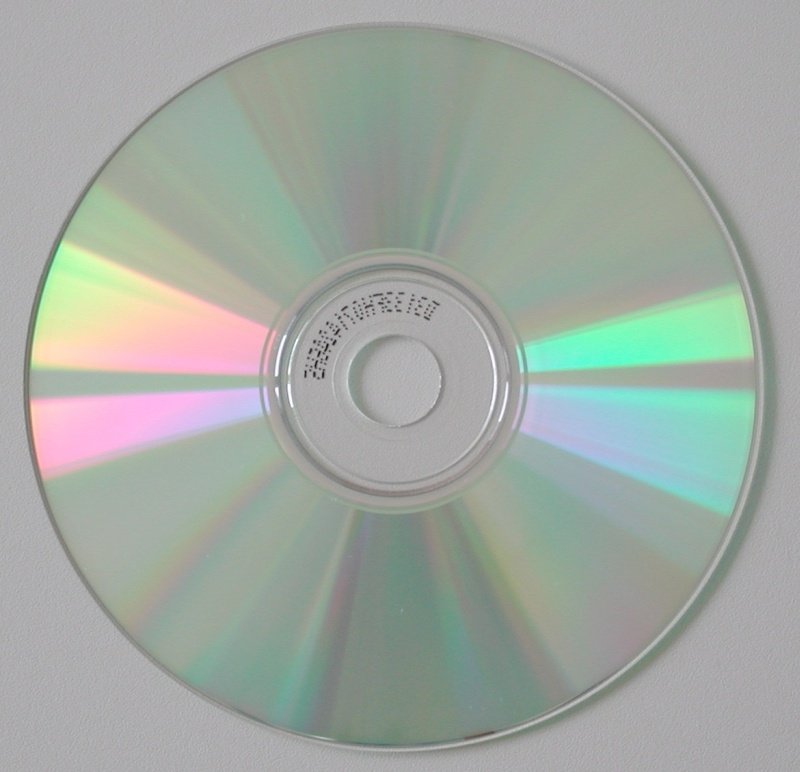
\includegraphics[width=\textwidth]{figures/cdrom.jpg}
\caption{The CD-ROM of this project}
\label{fig:cdrom}
\end{figure}

